\documentclass[3p, authoryear]{elsarticle} %review=doublespace preprint=single 5p=2 column
%%% Begin My package additions %%%%%%%%%%%%%%%%%%%
\usepackage[hyphens]{url}

  \journal{Findings} % Sets Journal name


\usepackage{lineno} % add
\providecommand{\tightlist}{%
  \setlength{\itemsep}{0pt}\setlength{\parskip}{0pt}}

\usepackage{graphicx}
%%%%%%%%%%%%%%%% end my additions to header

\usepackage[T1]{fontenc}
\usepackage{lmodern}
\usepackage{amssymb,amsmath}
\usepackage{ifxetex,ifluatex}
\usepackage{fixltx2e} % provides \textsubscript
% use upquote if available, for straight quotes in verbatim environments
\IfFileExists{upquote.sty}{\usepackage{upquote}}{}
\ifnum 0\ifxetex 1\fi\ifluatex 1\fi=0 % if pdftex
  \usepackage[utf8]{inputenc}
\else % if luatex or xelatex
  \usepackage{fontspec}
  \ifxetex
    \usepackage{xltxtra,xunicode}
  \fi
  \defaultfontfeatures{Mapping=tex-text,Scale=MatchLowercase}
  \newcommand{\euro}{€}
\fi
% use microtype if available
\IfFileExists{microtype.sty}{\usepackage{microtype}}{}
\usepackage{natbib}
\bibliographystyle{apalike}
\usepackage{longtable,booktabs,array}
\usepackage{calc} % for calculating minipage widths
% Correct order of tables after \paragraph or \subparagraph
\usepackage{etoolbox}
\makeatletter
\patchcmd\longtable{\par}{\if@noskipsec\mbox{}\fi\par}{}{}
\makeatother
% Allow footnotes in longtable head/foot
\IfFileExists{footnotehyper.sty}{\usepackage{footnotehyper}}{\usepackage{footnote}}
\makesavenoteenv{longtable}
\ifxetex
  \usepackage[setpagesize=false, % page size defined by xetex
              unicode=false, % unicode breaks when used with xetex
              xetex]{hyperref}
\else
  \usepackage[unicode=true]{hyperref}
\fi
\hypersetup{breaklinks=true,
            bookmarks=true,
            pdfauthor={},
            pdftitle={Vehicle Crash Severity Correlating Factors},
            colorlinks=false,
            urlcolor=blue,
            linkcolor=magenta,
            pdfborder={0 0 0}}
\urlstyle{same}  % don't use monospace font for urls

\setcounter{secnumdepth}{5}
% Pandoc toggle for numbering sections (defaults to be off)

% Pandoc citation processing

% Pandoc header
\usepackage{booktabs}
\usepackage{booktabs}
\usepackage{longtable}
\usepackage{array}
\usepackage{multirow}
\usepackage{wrapfig}
\usepackage{float}
\usepackage{colortbl}
\usepackage{pdflscape}
\usepackage{tabu}
\usepackage{threeparttable}
\usepackage{threeparttablex}
\usepackage[normalem]{ulem}
\usepackage{makecell}
\usepackage{xcolor}



\begin{document}
\begin{frontmatter}

  \title{Vehicle Crash Severity Correlating Factors}
    \author[Brigham Young University]{Samuel Runyan\corref{1}}
   \ead{samyan@byu.edu} 
      \address[Brigham Young University]{Civil and Environmental Engineering Department, 430 Engineering Building, Provo, Utah 84602}
    
  \begin{abstract}
  This is where the abstract should go.
  \end{abstract}
   \begin{keyword} Highway Safety Analysis Crash Severity Statistical Correlation\end{keyword}
 \end{frontmatter}

\hypertarget{intro}{%
\section{QUESTIONS}\label{intro}}

Research in network screening for highway safety analysis is continually developing and improving as data processing technologies and understanding of crash data improve. However, a major difficulty with most current network screening methodologies is that they do not account for the influence of crash severity towards the overall potential for safety improvement (PSI) of roadways. Therefore, it is valuable to use a crash severity-weighted approach when performing network screening. \citet{yasmin2018} and \citet{afghari2020} assert that a joint crash count with crash severity model is best suited to identify sites with the most PSI because of the correlation between crash counts and crash severity. As part of this joint model, it may be helpful to consider other factors which may contribute to the crash severity distribution at a given site.

The purpose of this article is to identify any additional factors that may correlate to crash severity such as the manner of collision, the presence of pedestrians, the light conditions, and so on. The results of this article will help determine which of these factors are significant enough to include in severity-weighted network screening. In the past, many network screening models have been limited by precedent, but this research aims to expound on and improve these tried and tested methods. With better understanding of how crash factors relate to crash severity, it may be possible to more proactively prevent severe crashes rather than waiting for them to happen before they can be modeled.

\hypertarget{methods}{%
\section{METHODS}\label{methods}}

In order to determine the correlation between crash severity and manner of collision, pedestrian presence, etc\ldots{}
the Pearson correlation were determined for different factors. The
equation below demonstrates how to calculate the Pearson correlation factor
using two potentially correlated variables \eqref{eq:pearson}. In this experiment,
manner of collision, presence of pedestrians, and other factors were compared to crash severity to determine correlation factors.

\begin{equation}
  \rho = \frac{\text{cov}(X,Y)}{\sigma_x \sigma_y}
  \label{eq:pearson}
\end{equation}

Crash data was retrieved from the Utah Department of Transportation (UDOT). The data was collected through police reports and contains information about crash severity, manner of collision, and other details. In order to perform analysis on the data, four crash files concerning crashes, crash details, location, and vehicles involved had to be combined. Then the the crashes were separated by segments and intersections to allow for consistent analysis.

The data was then filtered to compare the crash severities and manners of collision for segments and intersections separately.
Table \ref{tab:segManner} shows the Pearson correlation factors between crash severities and manners of collision for segments.

\begin{table}

\caption{\label{tab:segManner}Correlation Matrix for Crash Severity and Manner of Collision at Segments}
\centering
\resizebox{\linewidth}{!}{
\begin{tabular}[t]{>{\raggedright\arraybackslash}p{8em}>{\centering\arraybackslash}p{8em}>{\centering\arraybackslash}p{8em}>{\centering\arraybackslash}p{8em}>{\centering\arraybackslash}p{8em}>{\centering\arraybackslash}p{8em}>{\centering\arraybackslash}p{8em}>{\centering\arraybackslash}p{8em}}
\toprule
  & Severity 1 (Property Damage Only) & Severity 2 (Possible Injury) & Severity 3 (Suspected Minor Injury) & Severity 4 (Suspected Major Injury) & Severity 5 (Fatal Injury) & Severities 3-5 (Injury) & Severities 4-5 (Severe Injury)\\
\midrule
\cellcolor{gray!6}{\textbf{Angle}} & \cellcolor{gray!6}{0.48} & \cellcolor{gray!6}{0.56} & \cellcolor{gray!6}{0.62} & \cellcolor{gray!6}{0.42} & \cellcolor{gray!6}{0.18} & \cellcolor{gray!6}{0.60} & \cellcolor{gray!6}{0.41}\\
\addlinespace
\textbf{Front to Rear} & 0.87 & 0.94 & 0.73 & 0.38 & 0.14 & 0.67 & 0.36\\
\addlinespace
\cellcolor{gray!6}{\textbf{Head on}} & \cellcolor{gray!6}{0.45} & \cellcolor{gray!6}{0.50} & \cellcolor{gray!6}{0.55} & \cellcolor{gray!6}{0.39} & \cellcolor{gray!6}{0.30} & \cellcolor{gray!6}{0.55} & \cellcolor{gray!6}{0.41}\\
\addlinespace
\textbf{Sideswipe in the Same Direction} & 0.88 & 0.86 & 0.74 & 0.44 & 0.20 & 0.70 & 0.43\\
\addlinespace
\cellcolor{gray!6}{\textbf{Sideswipe in the Opposite Direction}} & \cellcolor{gray!6}{0.34} & \cellcolor{gray!6}{0.35} & \cellcolor{gray!6}{0.46} & \cellcolor{gray!6}{0.39} & \cellcolor{gray!6}{0.29} & \cellcolor{gray!6}{0.48} & \cellcolor{gray!6}{0.41}\\
\addlinespace
\textbf{Collision with Parked Vehicle} & 0.38 & 0.36 & 0.42 & 0.30 & 0.22 & 0.42 & 0.32\\
\addlinespace
\cellcolor{gray!6}{\textbf{Rear to Side}} & \cellcolor{gray!6}{0.14} & \cellcolor{gray!6}{0.15} & \cellcolor{gray!6}{0.15} & \cellcolor{gray!6}{0.12} & \cellcolor{gray!6}{0.09} & \cellcolor{gray!6}{0.16} & \cellcolor{gray!6}{0.13}\\
\addlinespace
\textbf{Rear to Rear} & 0.20 & 0.21 & 0.19 & 0.08 & 0.08 & 0.18 & 0.09\\
\addlinespace
\cellcolor{gray!6}{\textbf{Single Vehicle Crash}} & \cellcolor{gray!6}{0.71} & \cellcolor{gray!6}{0.49} & \cellcolor{gray!6}{0.63} & \cellcolor{gray!6}{0.62} & \cellcolor{gray!6}{0.49} & \cellcolor{gray!6}{0.68} & \cellcolor{gray!6}{0.67}\\
\bottomrule
\end{tabular}}
\end{table}

\begin{table}

\caption{\label{tab:intManner}Correlation Matrix for Crash Severity and Manner of Collision at Intersections}
\centering
\resizebox{\linewidth}{!}{
\begin{tabular}[t]{>{\raggedright\arraybackslash}p{8em}>{\centering\arraybackslash}p{8em}>{\centering\arraybackslash}p{8em}>{\centering\arraybackslash}p{8em}>{\centering\arraybackslash}p{8em}>{\centering\arraybackslash}p{8em}>{\centering\arraybackslash}p{8em}>{\centering\arraybackslash}p{8em}}
\toprule
  & Severity 1 (Property Damage Only) & Severity 2 (Possible Injury) & Severity 3 (Suspected Minor Injury) & Severity 4 (Suspected Major Injury) & Severity 5 (Fatal Injury) & Severities 3-5 (Injury) & Severities 4-5 (Severe Injury)\\
\midrule
\cellcolor{gray!6}{\textbf{Angle}} & \cellcolor{gray!6}{0.85} & \cellcolor{gray!6}{0.90} & \cellcolor{gray!6}{0.86} & \cellcolor{gray!6}{0.63} & \cellcolor{gray!6}{0.26} & \cellcolor{gray!6}{0.87} & \cellcolor{gray!6}{0.64}\\
\addlinespace
\textbf{Front to Rear} & 0.94 & 0.84 & 0.67 & 0.51 & 0.20 & 0.68 & 0.52\\
\addlinespace
\cellcolor{gray!6}{\textbf{Head on}} & \cellcolor{gray!6}{0.65} & \cellcolor{gray!6}{0.71} & \cellcolor{gray!6}{0.65} & \cellcolor{gray!6}{0.41} & \cellcolor{gray!6}{0.20} & \cellcolor{gray!6}{0.64} & \cellcolor{gray!6}{0.43}\\
\addlinespace
\textbf{Sideswipe in the Same Direction} & 0.83 & 0.70 & 0.52 & 0.40 & 0.22 & 0.53 & 0.42\\
\addlinespace
\cellcolor{gray!6}{\textbf{Sideswipe in the Opposite Direction}} & \cellcolor{gray!6}{0.66} & \cellcolor{gray!6}{0.68} & \cellcolor{gray!6}{0.59} & \cellcolor{gray!6}{0.43} & \cellcolor{gray!6}{0.18} & \cellcolor{gray!6}{0.60} & \cellcolor{gray!6}{0.44}\\
\addlinespace
\textbf{Collision with Parked Vehicle} & 0.30 & 0.33 & 0.23 & 0.20 & 0.07 & 0.24 & 0.20\\
\addlinespace
\cellcolor{gray!6}{\textbf{Rear to Side}} & \cellcolor{gray!6}{0.21} & \cellcolor{gray!6}{0.19} & \cellcolor{gray!6}{0.16} & \cellcolor{gray!6}{0.05} & \cellcolor{gray!6}{0.21} & \cellcolor{gray!6}{0.16} & \cellcolor{gray!6}{0.10}\\
\addlinespace
\textbf{Rear to Rear} & 0.09 & 0.06 & 0.04 & 0.06 & 0.05 & 0.05 & 0.07\\
\addlinespace
\cellcolor{gray!6}{\textbf{Single Vehicle Crash}} & \cellcolor{gray!6}{0.67} & \cellcolor{gray!6}{0.70} & \cellcolor{gray!6}{0.68} & \cellcolor{gray!6}{0.49} & \cellcolor{gray!6}{0.23} & \cellcolor{gray!6}{0.69} & \cellcolor{gray!6}{0.51}\\
\bottomrule
\end{tabular}}
\end{table}

The segmentation method used in this model is based on characteristics like AADT and length to facilitate homogeneous segments. Intersection related crashes were determined by estimating the location of the stop bar given approach speeds. Considering that the segments and intersection are homogeneous and consistent, it is possible to calculate correlation between crash severities and other factors.

(I hope to include correlation to other factors like the presence of bus stops and schools near intersections, but I have a little more to do to prepare that data.)

\begin{table}

\caption{\label{tab:segPed}Correlation Matrix for Crash Severity and Pedestrain Variables at Segments}
\centering
\resizebox{\linewidth}{!}{
\begin{tabular}[t]{>{\raggedright\arraybackslash}p{8em}>{\centering\arraybackslash}p{8em}>{\centering\arraybackslash}p{8em}>{\centering\arraybackslash}p{8em}>{\centering\arraybackslash}p{8em}cccc}
\toprule
  & Severity 1 (Property Damage Only) & Severity 2 (Possible Injury) & Severity 3 (Suspected Minor Injury) & Severity 4 (Suspected Major Injury) & Severity 5 (Fatal Injury) & Severities 3-5 (Injury) & Severities 4-5 (Severe Injury) & Total Crashes\\
\midrule
\cellcolor{gray!6}{\textbf{Pedestrian Involved}} & \cellcolor{gray!6}{0.33} & \cellcolor{gray!6}{0.40} & \cellcolor{gray!6}{0.47} & \cellcolor{gray!6}{0.32} & \cellcolor{gray!6}{0.27} & \cellcolor{gray!6}{0.47} & \cellcolor{gray!6}{0.35} & \cellcolor{gray!6}{0.37}\\
\addlinespace
\textbf{Pedacycle Involved} & 0.22 & 0.29 & 0.35 & 0.21 & 0.10 & 0.33 & 0.21 & 0.25\\
\addlinespace
\cellcolor{gray!6}{\textbf{Motorcycle Involved}} & \cellcolor{gray!6}{0.44} & \cellcolor{gray!6}{0.43} & \cellcolor{gray!6}{0.55} & \cellcolor{gray!6}{0.49} & \cellcolor{gray!6}{0.31} & \cellcolor{gray!6}{0.57} & \cellcolor{gray!6}{0.51} & \cellcolor{gray!6}{0.46}\\
\addlinespace
\textbf{Number of Schools Within 1000 Feet} & 0.01 & 0.05 & 0.04 & -0.01 & -0.04 & 0.02 & -0.02 & 0.02\\
\addlinespace
\cellcolor{gray!6}{\textbf{Presence of Schools Within 1000 Feet}} & \cellcolor{gray!6}{0.13} & \cellcolor{gray!6}{0.16} & \cellcolor{gray!6}{0.17} & \cellcolor{gray!6}{0.09} & \cellcolor{gray!6}{0.01} & \cellcolor{gray!6}{0.16} & \cellcolor{gray!6}{0.08} & \cellcolor{gray!6}{0.14}\\
\addlinespace
\textbf{Number of Transit Stops Within 1000 Feet} & 0.13 & 0.21 & 0.23 & 0.08 & 0.00 & 0.20 & 0.07 & 0.16\\
\addlinespace
\cellcolor{gray!6}{\textbf{Presence of Transit Stops Within 1000 Feet}} & \cellcolor{gray!6}{0.28} & \cellcolor{gray!6}{0.35} & \cellcolor{gray!6}{0.31} & \cellcolor{gray!6}{0.11} & \cellcolor{gray!6}{0.00} & \cellcolor{gray!6}{0.27} & \cellcolor{gray!6}{0.09} & \cellcolor{gray!6}{0.30}\\
\bottomrule
\end{tabular}}
\end{table}

\begin{table}

\caption{\label{tab:intPed}Correlation Matrix for Crash Severity and Pedestrian Variables at Intersections}
\centering
\resizebox{\linewidth}{!}{
\begin{tabular}[t]{>{\raggedright\arraybackslash}p{8em}>{\centering\arraybackslash}p{8em}>{\centering\arraybackslash}p{8em}>{\centering\arraybackslash}p{8em}>{\centering\arraybackslash}p{8em}cccc}
\toprule
  & Severity 1 (Property Damage Only) & Severity 2 (Possible Injury) & Severity 3 (Suspected Minor Injury) & Severity 4 (Suspected Major Injury) & Severity 5 (Fatal Injury) & Severities 3-5 (Injury) & Severities 4-5 (Severe Injury) & Total Crashes\\
\midrule
\cellcolor{gray!6}{\textbf{Pedestrian Involved}} & \cellcolor{gray!6}{0.49} & \cellcolor{gray!6}{0.56} & \cellcolor{gray!6}{0.55} & \cellcolor{gray!6}{0.41} & \cellcolor{gray!6}{0.19} & \cellcolor{gray!6}{0.56} & \cellcolor{gray!6}{0.42} & \cellcolor{gray!6}{0.54}\\
\addlinespace
\textbf{Pedacycle Involved} & 0.41 & 0.51 & 0.57 & 0.37 & 0.12 & 0.57 & 0.37 & 0.47\\
\addlinespace
\cellcolor{gray!6}{\textbf{Motorcycle Involved}} & \cellcolor{gray!6}{0.61} & \cellcolor{gray!6}{0.61} & \cellcolor{gray!6}{0.59} & \cellcolor{gray!6}{0.47} & \cellcolor{gray!6}{0.16} & \cellcolor{gray!6}{0.60} & \cellcolor{gray!6}{0.47} & \cellcolor{gray!6}{0.64}\\
\addlinespace
\textbf{Number of Schools Within 1000 Feet} & -0.07 & -0.08 & -0.08 & -0.02 & -0.05 & -0.08 & -0.03 & -0.08\\
\addlinespace
\cellcolor{gray!6}{\textbf{Presence of Schools Within 1000 Feet}} & \cellcolor{gray!6}{-0.03} & \cellcolor{gray!6}{-0.04} & \cellcolor{gray!6}{-0.05} & \cellcolor{gray!6}{0.02} & \cellcolor{gray!6}{-0.03} & \cellcolor{gray!6}{-0.04} & \cellcolor{gray!6}{0.01} & \cellcolor{gray!6}{-0.04}\\
\addlinespace
\textbf{Number of Transit Stops Within 1000 Feet} & 0.15 & 0.19 & 0.20 & 0.14 & -0.01 & 0.19 & 0.12 & 0.17\\
\addlinespace
\cellcolor{gray!6}{\textbf{Presence of Transit Stops Within 1000 Feet}} & \cellcolor{gray!6}{0.27} & \cellcolor{gray!6}{0.32} & \cellcolor{gray!6}{0.33} & \cellcolor{gray!6}{0.19} & \cellcolor{gray!6}{0.07} & \cellcolor{gray!6}{0.32} & \cellcolor{gray!6}{0.19} & \cellcolor{gray!6}{0.30}\\
\bottomrule
\end{tabular}}
\end{table}

\hypertarget{findings}{%
\section{FINDINGS}\label{findings}}

The Pearson correlation factors for severe injury crashes and manner of collision are summarized in Figure \ref{fig:mannerSeverityCorr}. That plot is created with the `ggplot2()' package and function.

\begin{center}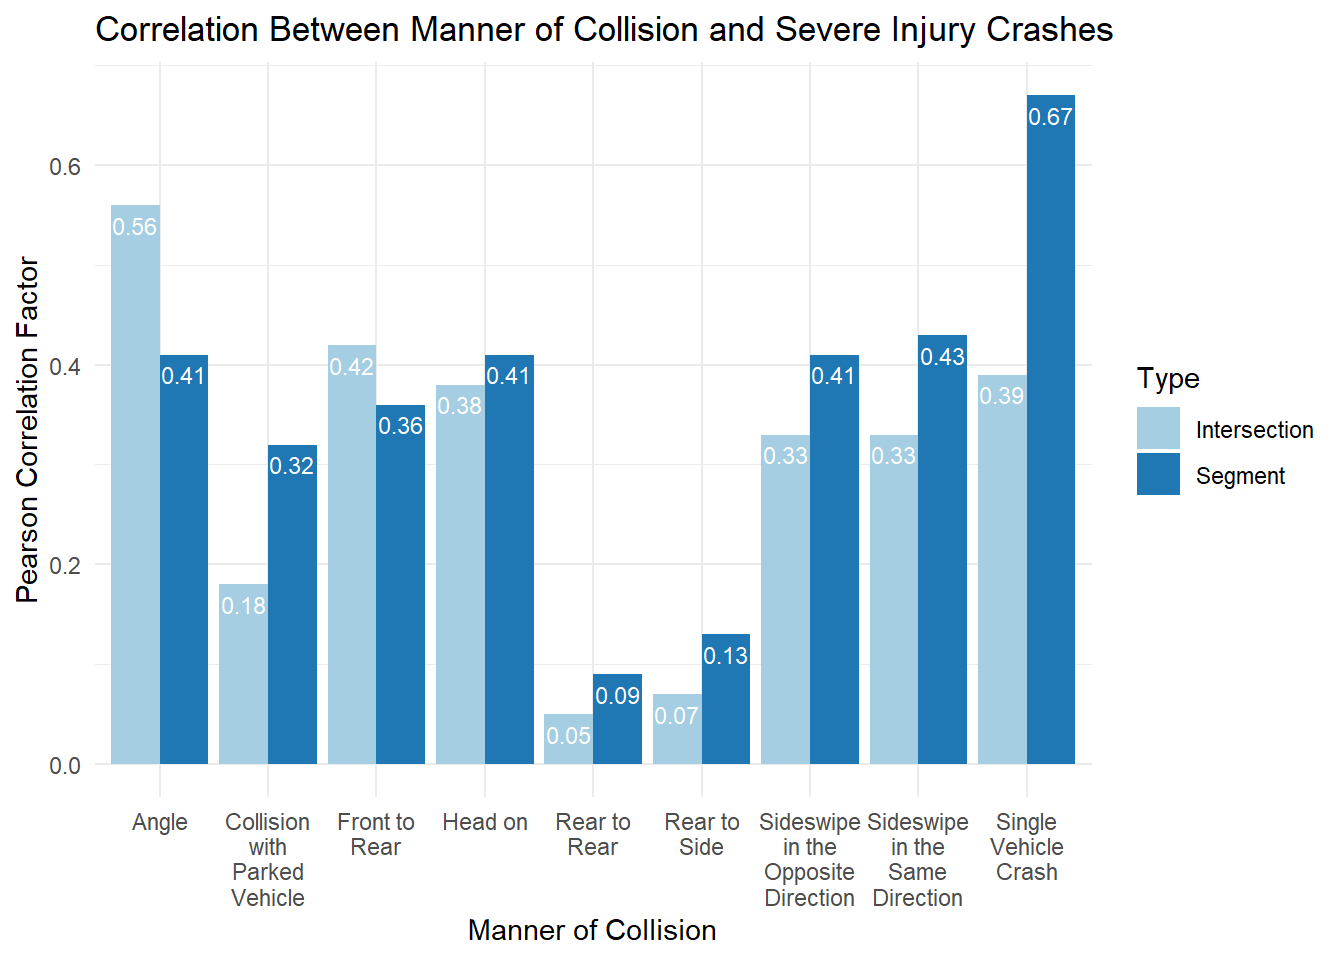
\includegraphics{Crash_Severity_Correlations_files/figure-latex/mannerSeverityCorr-1} \end{center}

Mannners of collision that have a higher correlation factor regarding severe injury crashes are understood to be more severe. First, we notice that single vehicle crashes are much more severe for segments than for intersections. These are a broad category of crashes, so it is difficult to determine the cause of this outright. We also notice that angle crashes tend to be more severe than other crashes, especially at intersections. Furthermore, collisions with parked cars and sideswipes tend to be more severe at segments than intersections while front to rear and head on crashes are similarly severe for both. The only crashes that are very unlikely to be severe are rear to rear and rear to side crashes.

Unfortunately, these manners of collision do not account for factors such as pedestrian involvement, so it is difficult to determine the impact of pedestrians on crash severity from this data alone. That is why it is useful to evaluate the correlation between crash severity and crashes near schools, bus stops, or crashes which involved pedestrians since these will give a better indication to how varying levels of pedestrian involvement affect crash severity.

\begin{center}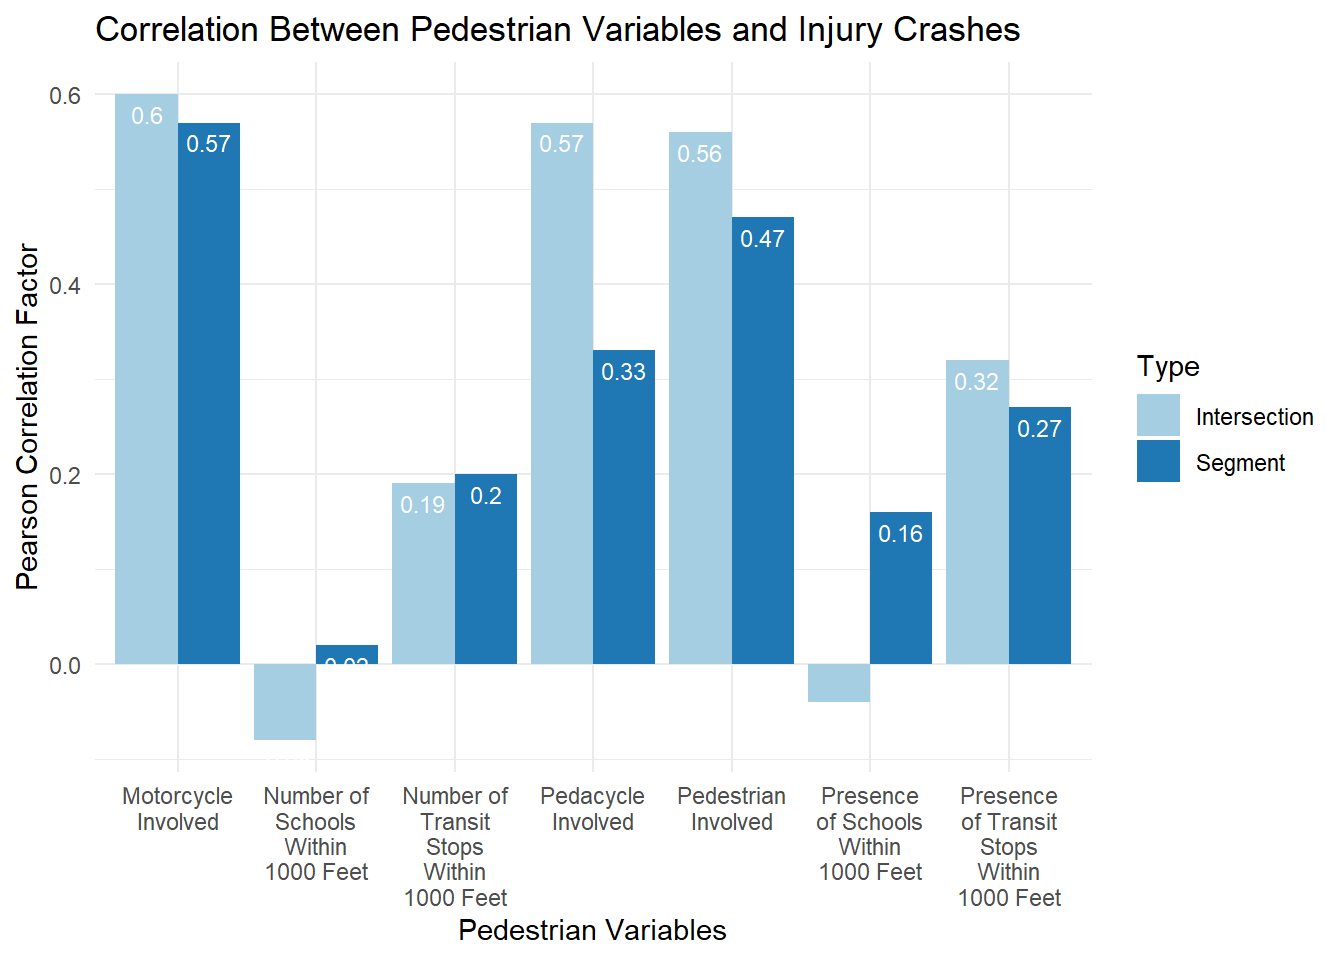
\includegraphics{Crash_Severity_Correlations_files/figure-latex/pedSeverityCorr-1} \end{center}

This analysis could be used to implement more informed safety measures with crash severity in mind. Knowing which types of crashes are more likely to lead to severe injury will help officials design roadways and inform the public to better avoid these types of collisions. This has applications in automated vehicles as well because engineers can design vehicles to put special emphasis on avoiding the types of crashes that are more likely to lead to severe injury.

\bibliography{book.bib}


\end{document}
